%%%%%%%%%%%%%%%%%%%%%%%%%%%%%%%%%%%%%%%%%%%%%%%%%%%%%%%%%%%%%%%%%%%%%%%%
%                                                                      %
%     File: Thesis_Introduction.tex                                    %
%     Tex Master: Thesis.tex                                           %
%                                                                      %
%     Author: Rui Santiago                         			   %
%     Last modified : 2 Junho 2015                         		   %
%                                                                      %
%%%%%%%%%%%%%%%%%%%%%%%%%%%%%%%%%%%%%%%%%%%%%%%%%%%%%%%%%%%%%%%%%%%%%%%%
\chapter{Arquitectura do Versat}
\label{chapter:Arquitectura do Versat}
\setlength{\parskip}{0 cm}
%O sistema num chip em inglês System On Chip \acrlong{soc} é um chip integrado que tem integrado todas as funcionalidades de computador ou de um sistema electrónico, num único chip. Um \acrshort{soc} é constituído tipicamente por vários elementos interligados entre si por um barramento. Os elementos podem ser separados por grupos conformes os seus principais funcionalidades, os principais grupos são os seguintes: processamento, memoria, fontes de \textcolor[rgb]{1,0,0}{timing}, periféricos, interfaces externas, interfaces analógicas e gestores de energia. Na figura \ref{figures:ARM} pode se um exemplo de um diagrama de blocos de um \acrshort{soc}, onde se pode o barramento ligação dos elementos.
O Versat usa uma arquitectura {\it Coarse Grain Reconfigurable Arrays} (CGRAs). As arquitecturas CGRA surgiram com o objectivo de reduzir a complexidade, o tempo de configuração e o tempo de compilação em relação às arquitecturas FPGA. 

Todas as CGRAs possuem elementos de processamento (ALUs, multiplicadores, etc), onde são realizadas as operações. Também possuem uma rede de interconexão, que é usada para unir os vários elementos de processamento e memórias que armazenam configurações da arquitectura. As CGRAs variam em relação ao tipo de unidades de processamento utlizadas e à respectiva rede de interconexão. 


Dado que os sistemas homogéneos causam um desperdício de recursos, o Versat usa unidades de processamento heterogéneas. 
Para a realização da interconexão, as estruturas com nós todos conectados uns com os outros têm sido evitadas, visto que têm escalabilidade pobre em termos de área, um atraso entre os nós maior e um consumo maior. 
No entanto, no caso do Versat é usada esta topologia, pois é privilegiada a flexibilidade de configuração face à escalabilidade. Cada sistema Versat utiliza um número reduzido de nós, prevendo-se que a escalabilidade passe pela utilização de multiplos sistemas Versat em vez de um sistema Versat de grandes dimensões.
O facto de ser utilizado um número reduzido de nós compensa o facto dos nós estarem todos interligados. 
Um número restrito de nós é usado também para evitar uma área muito grande. Note-se que a área varia quadraticamente com o número de ligações.



Numa tecnologia CMOS, a potência varia de acordo com a seguinte relação: 

%P $\propto$ CVfA                                                        (1)
\begin{equation} P \propto CV^{2}fA \end{equation}

onde:
\begin{itemize}
  \item P é a potência do circuito;
  \item C é a capacidade da porta;
  \item V é o VDD;
  \item f é a frequência de relógio;
  \item A é a área do circuito.
\end{itemize}

Assim pode pensar-se que a redução de potência pode conseguir-se por redução da frequência de trabalho e consequente redução da tensão de alimentação,
compensada pelo elevado grau de paralelismo possível durante a execução de programas no Versat.

%\begin{figure}[!htb]
 % \centering
 % 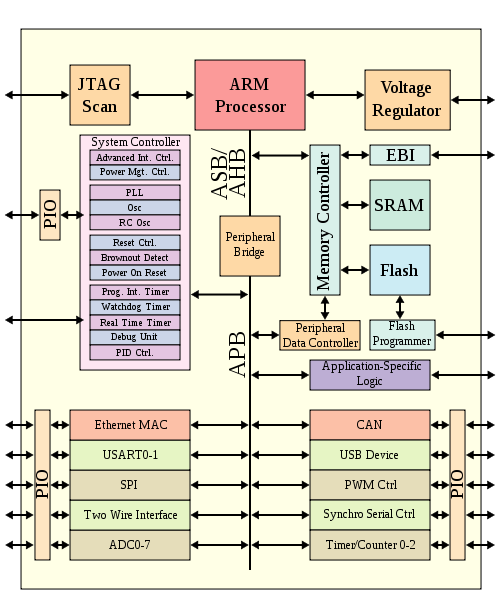
\includegraphics[width=0.5\textwidth]{Figures/ARM_SOC.png}
 % \caption[Diagrama de blocos de um soc ARM ]{Diagrama de blocos de um soc ARM }
 % \label{figures:ARM}
  %http://en.wikipedia.org/wiki/System_on_a_chip
%\end{figure}

%Os \acrshort{soc} têm uma vasta possibilidade de utilização desde um simples relógio até no mais avançado tecnologicamente como no desenvolvimentos de módulos para satélites, passando pela industria automóvel e com o aparecimento do arduino cada vez mais os \acrshort{soc} são utilizados em projetos de pequena escala desenvolvidos em casa, porque veio permitir a pessoas de com pouco ou nenhum conhecimento na área programar e efectuar debug no seu projecto com o \acrshort{soc}. A sua utilização traz vantagens com preço baixo, baixo consumo de energia e dimensões pequenas, como tudo o que existe também tem desvantagens sendo neste caso o baixo poder de calculo comparado com um computador. %http://www.extremetech.com/computing/126235-soc-vs-cpu-the-battle-for-the-future-of-computing

%Com uma área tão vasta de aplicações não é de estranhar que existam várias empresas \textcolor[rgb]{1,0,0}{a muito tempo} e varias startup no mercado a desenvolver \acrshort{soc} para fins totalmente distintos, cada empresa optimizando o seu para que foi desenvolvido.



% --------------------------------------------------------------------- 
\section{Modelo de Topo}
\label{section:Modelo de Topo}

O diagrama de topo do Versat é dado pela figura 3.1.

\begin{figure}[!htb]
  \centering
  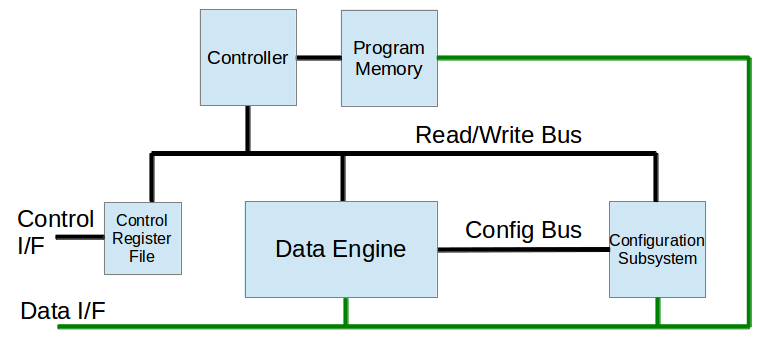
\includegraphics[height=80mm, width=165mm]{Figures/top.png}
  \caption[Esquema da unidade de topo.]{Esquema da unidade de topo.}  
  \label{fig:Esquema_Unidade_Topo}
\end{figure}

No Versat existem vários sub-componentes:

\begin{itemize}
  \item Data engine;
  \item Subsistema de configuração;
  \item Memória de instruções;
  \item Controlador;
  \item Ficheiro de registos de controlo;
  \item Descodificador de endereços;
  \item Sistema host-guest. 
\end{itemize}
%Uma startup no desenvolvimento de um projecto/produto necessita de um \acrshort{soc} para poder comercializar o seu produto. Na pesquisa do \acrshort{soc} ideal para o seu projecto encontram diferentes possibilidades, mas nenhuma preenchia todos os critérios pretendidos para o projecto. Como não foi encontrada uma solução ideal dos vários \acrshort{soc} disponíveis no mercado, a solução possível serias desenvolver o seu próprio \acrshort{soc} desenvolvido a medidas para o projecto.

O Versat é controlado centralmente pelo seu controlador. O controlador controla o barramento de Leitura/Escrita, que é usado para efectuar leitura/escrita nos registos dos outros sub-componentes. 


%\setlength{\parskip}{0 cm}



A interface de controlo é usada por um sistema {\it host}, que está a controlar o Versat. Os comandos são dados por um {\it host} e o Versat executa o que o {\it host} lhe ordena. Pela interface de controlo, são trocados preferencialmente comandos e informações de estado para indicar, por exemplo, o fim de algum comando executado. A troca de dados é realizada pela interface de dados. É também possível trocar dados pela interface de controlo, mas apenas quando a velocidade de transferência dos dados for pouco relevante. Por exemplo, caso o Versat esteja em modo de depuração, é usada a interface de controlo.

Existem dois tipos de barramentos de controlo possíveis de seleccionar: o barramento SPI e o barramento paralelo. 
O barramento SPI é usado quando se liga o Versat a um anfitrião externo, como por exemplo, um PC, para por exemplo, realizar a depuração de programas. O escravo SPI é o Versat, enquanto o mestre SPI é o anfitrião externo. 
O barramento paralelo é usado quando se liga o Versat a um anfitrião embebido. Este barramento está ligado ao ficheiro de registos de controlo e opera de uma forma simples e genérica. Pode ser necessário adaptar esta interface a um formato comercial, por exemplo, utilizando um barramento amba-AXI.


\section{Controlador}
\label{section:Controlador}

O controlador é descrito pela figura 3.2.

\begin{figure}[!htb]
  \centering
  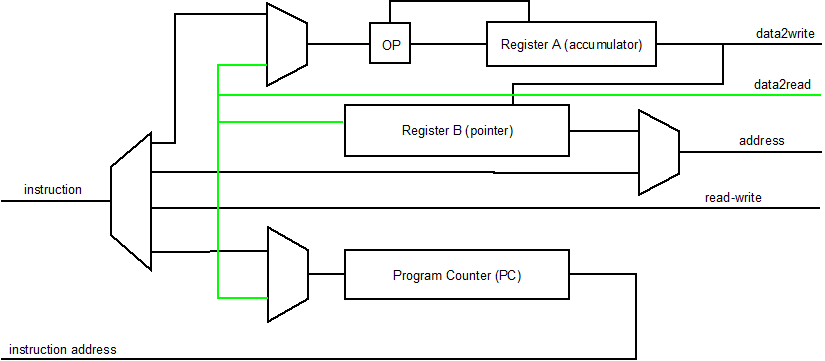
\includegraphics[height=110mm, width=155mm]{Figures/Controlador_MESMO.png}
  \caption[Esquema da unidade de controlo]{Esquema da unidade de controlo}  
  \label{fig:Esquema_Unidade_Controlo}
\end{figure}

\pagebreak

O controlador usa o barramento R/W para realizar leituras/escritas nos seus periféricos, que são módulos do Versat. A arquitectura do controlador do Versat é constituída por 3 registos:

\begin{itemize}
  \item Contador de programa;
  \item Acumulador (registo A);
  \item Apontador (registo B).
\end{itemize}

O contador de programa é usado como endereço da memória de instruções. A saída da memória de instruções contém a instrução que o controlador necessita de ler.

O Versat é uma arquitectura de acumulador. O registo A é o acumulador. O resultado de todas as operações realizadas pelo controlador vão parar ao acumulador, que armazena o valor.  
É no bloco OP que se efectuam as várias operações possíveis com o controlador. O bloco OP recebe como entrada o próprio acumulador e um dado de entrada de 32 {\it bits}. %onde se executa as instruções.  

O registo B é usado para endereçamento indirecto. O registo B guarda o endereço da próxima posição de memória a ler ou escrever numa instrução que utilize endereçamento indirecto. 


As funções principais do controlador são:

\begin{itemize}
  \item Comunicação com o sistema anfitrião;
  \item Implementação da estrutura de controlo dos procedimentos do Versat;
  \item Reconfiguração e controlo do Data Engine.
\end{itemize}

Caso o Versat esteja a trabalhar sozinho, em modo de depuração por exemplo, ele pode realizar o {\it upload}/{\it download} de dados e {\it upload} de procedimentos.

O controlador pode escrever na memória de instruções mas não pode ler da memória. Esta funcionalidade é usada para carregar procedimentos.
    
O controlador consegue ler e escrever no ficheiro de registos de controlo, que é partilhado com o sistema anfitrião. A função principal do ficheiro de registos de controlo é a de um canal de comunicação entre um anfitrião e o Versat. Os parâmetros necessários para correr os procedimentos no Versat são passados através deste canal.
    
O controlador pode escrever configurações parciais no subsistema de configuração de modo a reconfigurar o Data Engine. Também pode realizar pequenos cálculos que sejam necessários.

o conjunto de instruções executadas pelo controlador está descrito na tabela 3.1.

\pagebreak

\begin{table}[h!]
  \caption[Tabela das instruções assembly do Versat]{Tabela das instruções assembly do Versat}
  \begin{center}
    \begin{tabular}{|C{2cm}|c|c|c|}
      \hline
      {\bf Instruções} & {\bf Pseudo-código} \\
      \hline \hline
      nop & Nop \\
      \hline
      rdw & A $<$= (imm) \\
      \hline
      wrw & (imm) $<$= A \\
      \hline
      wrc & (imm1+imm2) $<$= A \\
      \hline
      rdwb & A $<$= (B) \\
      \hline 
      wrwb & (B) $<$= A \\
      \hline
      beqi & PC $<$= imm if regA=0\\
      \hline
      beq & PC $<$= (imm) if regA=0\\
      \hline
      bneqi & PC $<$= imm if regA!=0\\
      \hline
      bneq & PC $<$= (imm) if regA!=0\\
      \hline
      ldi & A $<$= imm \\
      \hline
      ldih & A[31:16] $<$= imm \\
      \hline
      add & A $<$= A + (imm) \\
      \hline
      addi & A $<$= A + imm\\
      \hline
      sub & A $<$= A - (imm)\\
      \hline 
      and & A $<$= A {\&} (imm) \\
     \hline
    \end{tabular}
  \end{center}
  \label{table:assembly_Versat}
\end{table}





%A startup no desenvolvimento de um projeto/produto necessita de um \acrshort{soc}, como se pode ver na figura \ref{grafos:problema} que tem de ter a capacidade de processamento necessária para efetuar a descodificação e codificação de dados que irá receber e enviar. O \acrshort{soc} desenvolvido tem de permitir que sejas ligado mais dois modelos assíncronos permitindo a recolha de dados no local para posterior envio dos dados pelo modelo de comunicação. O produto é para ser usado em locais de difíceis acessos este terá de ter um baixo consumo, permitindo que a bateria funcione o maior tempo possível. Para alem do mencionado anteriormente também necessita de duas interfaces de comunicação \acrlong{uart} e \acrlong{gpio}. 

%\begin{figure}[!htb]
 % \centering
 % 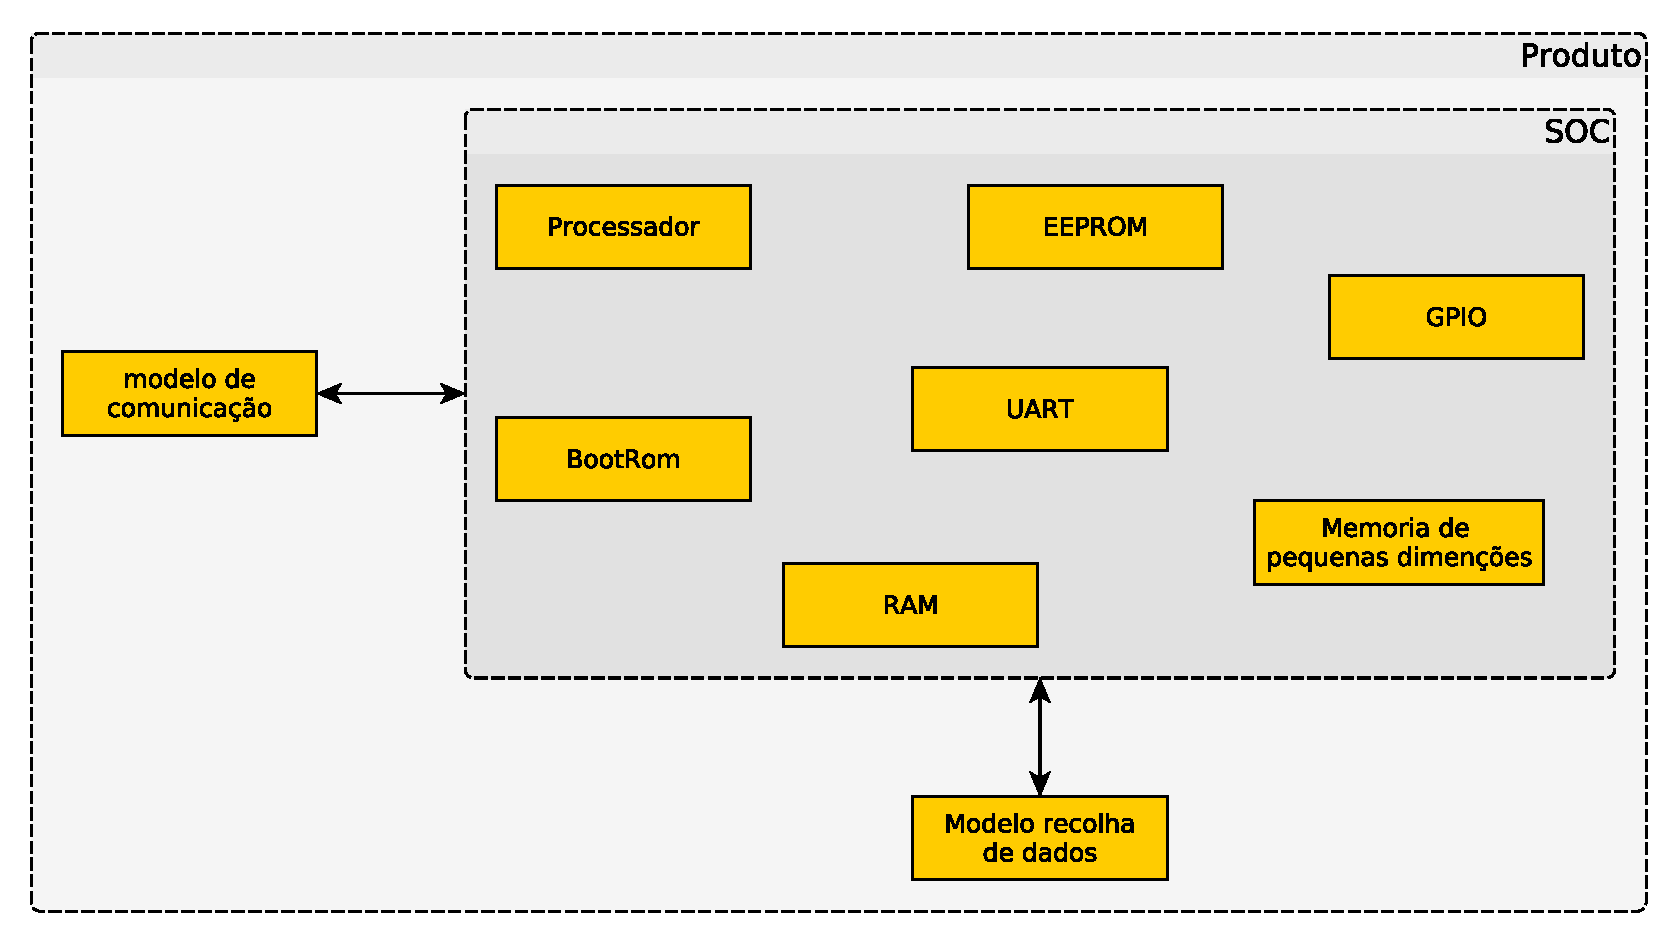
\includegraphics[width=0.5\textwidth]{grafos/problema.pdf}
 % \caption[SOC pretendido pela Startup]{SOC pretendido pela Startup}
 % \label{grafos:problema}
  %http://en.wikipedia.org/wiki/System_on_a_chip
%\end{figure}


\section{Data Engine}
\label{section:Data Engine}

O Data Engine é constituído por 15 unidades funcionais, organizadas como indicado na figura 3.3. A arquitectura usada tem 32 bits.



As memórias embebidas de porto duplo são memórias que têm um gerador de endereços por porto. É possível configurar cada um dos geradores de endereços de forma independente. Um gerador de endereços pode ser configurado com um número de iterações, período de cada iteração, incremento por ciclo, endereço de inicio e deslocamento entre períodos. 
As memórias podem ser configuradas para leitura ou escrita. No caso de serem configuradas para escrita, é necessário também configurar as entradas das memórias de modo a seleccionarem os dados certos.

As ALUs são unidades aritméticas lógicas que exercem diversas funções. As ALU-Lite executam apenas as primeiras 6 funções das ALUs, que são: 

\begin{itemize}
  \item OR lógico;
  \item AND lógico;
  \item NAND lógico;
  \item XOR lógico;
  \item Soma;
  \item Subtacção;
  \item Extensão de sinal de 8 para 32 bits;
  \item Extensão de sinal de 16 para 32 bits;
  \item SHIFT RIGHT aritmético;
  \item SHIFT RIGHT lógico;
  \item Comparação com sinal;
  \item Comparação sem sinal;
  \item Máximo; 
  \item Mínimo;
  \item Valor absoluto.
\end{itemize}

\begin{figure}[!htb]
  \centering
  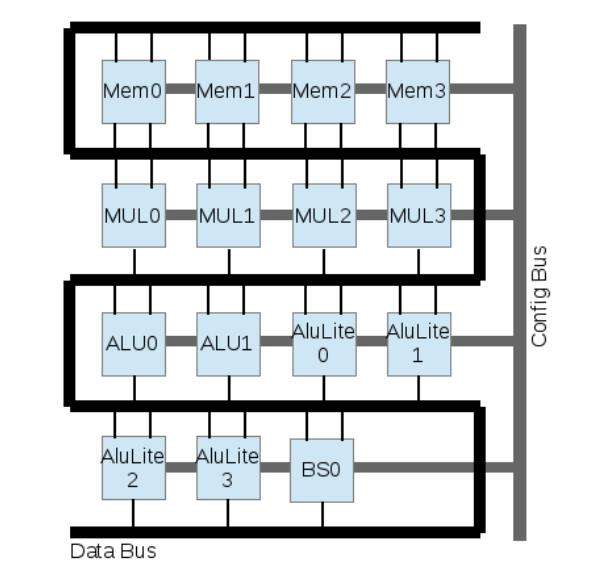
\includegraphics[height=130mm]{Figures/DataEngine.jpg}
  \caption[Esquema de ligações do Data Engine]{Esquema de ligações do Data Engine}  
  \label{fig:Esquema_ligacoes_DataEngine}
\end{figure}

Os multiplicadores efectuam uma multiplicação de dois operandos de 32 bits com um resultado de 64 bits, do qual só 32 bits são utilizados. É possível escolher se se quer a parte alta da multiplicação (bit 32 ao bit 63) ou a parte baixa (bit 0 ao bit 31). Também é possível escolher efectuar ou não a divisão por 2 do resultado final, o que ajuda quando se trabalha em notações de vírgula fixa.

Os {\it shifters} são unidades especializadas em deslocamento de bits. Um dos operandos é a palavra a deslocar e o outro operando é a magnitude do deslocamento. Os {\it shifters} são configurados com o sentido de deslocamento (esquerda ou direita) e o tipo de deslocamento (aritmético ou lógico).

Cada unidade de processamento contribui com 32 bits para o Data Bus. Cada unidade de processamento é capaz de seleccionar qualquer secção de 32 bits existente no Data Bus, o que permite que todas as unidades de processamento possam estar interligadas umas às outras. Isto facilita o trabalho do compilador, que não precisa de fazer {\it Place and Route}. 

As unidades de processamento são configuradas com o modo de operação e com as respectivas entradas. Não existem configurações globais, todas as configurações existentes são acerca de cada FU independente. Cada conjunto de unidades de processamento configuradas origina um datapath para uma tarefa específica.


Se num {\it datapath} estiverem várias memórias, as memórias vão trabalhar em sincronismo. Se existirem recursos suficientes, mais do que um {\it datapath} pode executar em paralelo, permitindo realizar paralelismo ao nível de tarefa. 

Para controlar o Data Engine, é necessário atribuir valores no seu registo de controlo, tal como descrito na tabela~\ref{tab:de_ctr_reg}. Pode essencialmente inicializar-se as unidades de processamento (bit 0, Init) ou manda-las correr (bit 1, Run). 
Os restantes bits deste registo (bit 2 a 20) indicam quais as unidades de processamento a inicializar ou correr. A inicialização de memórias tem como resultado o carregamento das configurações dos registos de endereços. A inicialização de outras unidades funcionais têm como resultado o anulamento do valor de saída.
Mandar correr as memórias faz iniciar a geração de endereços nas memórias indicadas. Mandar correr qualquer outra unidade de processamento tem apenas o efeito de anular as suas saídas inicialmente. 

\begin{table}[!htbp]
   \caption{Registo de controlo do Data Engine.}
  \centering
    \begin{tabular}{|p{1.5cm}|p{7cm}|}
    \hline 
    {\bf Bit} & {\bf Descrição} \\
    \hline \hline 
     0 & Init \\
    \hline
     1 & Run \\
    \hline
     2 & BS0 \\
    \hline
     3 & Mult3 \\
    \hline
     4 &  Mult2\\
    \hline
     5 &  Mult1  \\
    \hline
     6 & Mult0 \\
    \hline
     7 & ALULite3 \\
    \hline
     8 & ALULite2 \\
    \hline
     9 &  ALULite1\\
    \hline
     10 & ALULite0 \\
    \hline
     11 & ALU1 \\
    \hline
     12 & ALU0\\
    \hline
     13 & MEM3B \\
    \hline
     14 & MEM3A \\
    \hline
     15 &  MEM2B\\
    \hline
     16 &  MEM2A\\
    \hline
     17 &  MEM1B\\
    \hline
     18 &  MEM1A\\
    \hline
     19 &  MEM0B\\
    \hline
     20 &  MEM0A\\
    \hline
     21-31 & Reserved \\
    \hline
    \end{tabular}
  \label{tab:de_ctr_reg}
\end{table}

Quando se manda correr o Data Engine é necessário saber quando a sua operação termina. Para tal usa-se o registo de estado do Versat descrito na tabela~\ref{tab:de_stat_reg}. Este registo indica quais as memórias que terminaram a sua sequência de endereços.


\begin{table}[!htbp]
  \centering
  \caption{DE status register.}
    \begin{tabular}{|p{1.5cm}|p{7cm}|}
    \hline 
    {\bf Bit} & {\bf Description} \\
    \hline \hline 
     0 & MEM0B done \\
    \hline
     1 & MEM0A done\\
    \hline
     2 & MEM1B done \\
    \hline
     3 & MEM1A done \\
    \hline
     4 & MEM2B done \\
    \hline
     5 & MEM2A done  \\
    \hline
     6 & MEM3B done \\
    \hline
     7 & MEM3A done \\
    \hline
     8-31 & Reserved \\
    \hline

    \end{tabular}
  \label{tab:de_stat_reg}
\end{table}


\section{Subsistema de configuração}
\label{section:Subsistema de configuracao}

O subsistema de configuração é um sistema de memória onde as configurações do Data Engine estão guardadas. 

A configuração principal está guardada num registo parcialmente endereçado. Existe também uma réplica do registo de configuração principal (registo sombra) que permite manter a configuração do Data Engine enquanto que o registo de configuração principal é modificado para conter a próxima configuração. 
Existe também uma memória de configurações que permite armazenar configurações utilizadas frequentemente. Deste modo, após a escrita de uma configuração para o registo principal, e após a sua utilização no Data Engine, pode-se guardar o seu valor na memória de configurações para reutilização mais tarde.




\section{Memória de instruções}
\label{section:Memoria de instrucoes}

A memória de instruções é constituída por uma memória RAM e uma memória ROM. A memória RAM tem 2048 posições enquanto que a ROM tem 256 posições. No futuro poderá ser necessário aumentar o tamanho da memória, ou transforma-la numa cache, pois o uso de compiladores pode produzir código pouco optimizado.

O carregamento das instruções realiza-se numa fase de {\it setup}, antes de se usar o Versat. O carregamento das instruções é feita através da interface de dados entre o controlador do Versat e o exterior. 

A ROM (também designada de boot ROM) contém um programa fixo para carregamento de programas do Versat, dados e para executar programas previamente carregados. A boot ROM também pode ser usada para descarregar dados calculados pelo Versat. A RAM é usada após o carregamento do programa, para executar esse mesmo programa. 


\cleardoublepage






%Os principais desafios desta dissertação consiste no desenvolvimento de um sistema sintetizável que preencha todas as necessidades mencionadas pela startup.

%Desenvolver uma interface assíncrona necessária para a comunicação entre o \acrshort{soc} e os modelos de comunicação e de recolha de dados a ser desenvolvido pela startup.

%A criação de uma bootrom que carregua para a memoria principal o programa que se encontra na EEPROM. Ainda testa o mau funcionamento da EEPROM ou da memoria principal notificando o utilizador. 
